\documentclass[a4paper]{book}
\usepackage[utf8]{inputenc}
\usepackage[hidelinks]{hyperref}
\usepackage{pdfpages}
\usepackage{fullpage}
\usepackage{fancyhdr}
\usepackage{xcolor}
\usepackage{graphicx}
\usepackage{wrapfig}
\usepackage{baskervald}
\usepackage{geometry}
\usepackage{multicol}
\fancyhead{}
\fancyfoot[LE,RO]{\thepage}
\cfoot{}
\fancyfoot[LO,RE]{Scheme and Functional Programming Workshop 2017}
\renewcommand{\headrulewidth}{0.0pt}
\date{September 3rd, 2017}
\author{Nada Amin \and Fran\c{c}ois-Ren\'e Rideau}
\begin{document}
\frontmatter
\setcounter{page}{3}  % pages 1+2 to be added by TR editor
\newgeometry{textheight=8.5in,hmargin=20mm}
\chapter*{Preface}
This report aggregates the papers presented at the eigtheenth annual Scheme and
Functional Programming Workshop, hosted on September 3rd, 2017 in Oxford,
UK and co-located with the twenty-second International
Conference on Functional Programming.

\vspace{5pt}
\noindent
The Scheme and Functional Programming Workshop is held every year to provide an
opportunity for researchers and practitioners using Scheme and related
functional programming languages like Racket, Clojure, and Lisp, to share
research findings and discuss the future of the Scheme programming language.

\vspace{5pt}
\noindent
Two full papers and three lightning talks were submitted to the workshop, and each submission was reviewed by
three members of the program committee.  After deliberation, all submissions
were accepted to the workshop.

\vspace{5pt}
\noindent
In addition to the two full papers and three lightning talks presented
\begin{itemize}
\item Sam Tobin-Hochstadt gave an invited keynote speech entitled \textit{From Scheme to Typed Racket},
\item a panel including Michael Ballantyne, Arthur Gleckler, Kathy Gray, Alaric Snell-Pym, Andy Wingo as well as a lively audience debated on the future of Scheme,
\item Alaric Snell-Pym presented an update on the R7RS standardization process, and
\item Matt Might gave a closing invited talk on Precision Medecine.
\end{itemize}

\vspace{5pt}
\noindent
Thanks to all presenters, panelists, participants, and members of the
program committee.

\section*{Program Committee}
\begin{multicols}{2}
\noindent
Barış Aktemur, Ozyegin University\\
Nada Amin, University of Cambridge (General Chair)\\
Kenichi Asai, Ochanomizu University\\
Eli Barzilay, Microsoft\\
Felix S Klock II, Mozilla Research\\
Jay McCarthy, University of Massachusetts Lowell\\
Christian Queinnec, Sorbonne University\\
François-René Rideau, Metaphor (Program Chair)\\
\end{multicols}
\section*{Steering Committee}
\begin{multicols}{2}
\noindent
Will Clinger, Northeastern University\\
Marc Feeley, Universit\'{e} de Montr\'{e}al\\
Dan Friedman, Indiana University\\
Olin Shivers, Northeastern University\\
Will Byrd, University of Alabama at Birmingham\\
\end{multicols}
\tableofcontents
\mainmatter
\newgeometry{textheight=9.5in,hmargin=20mm}

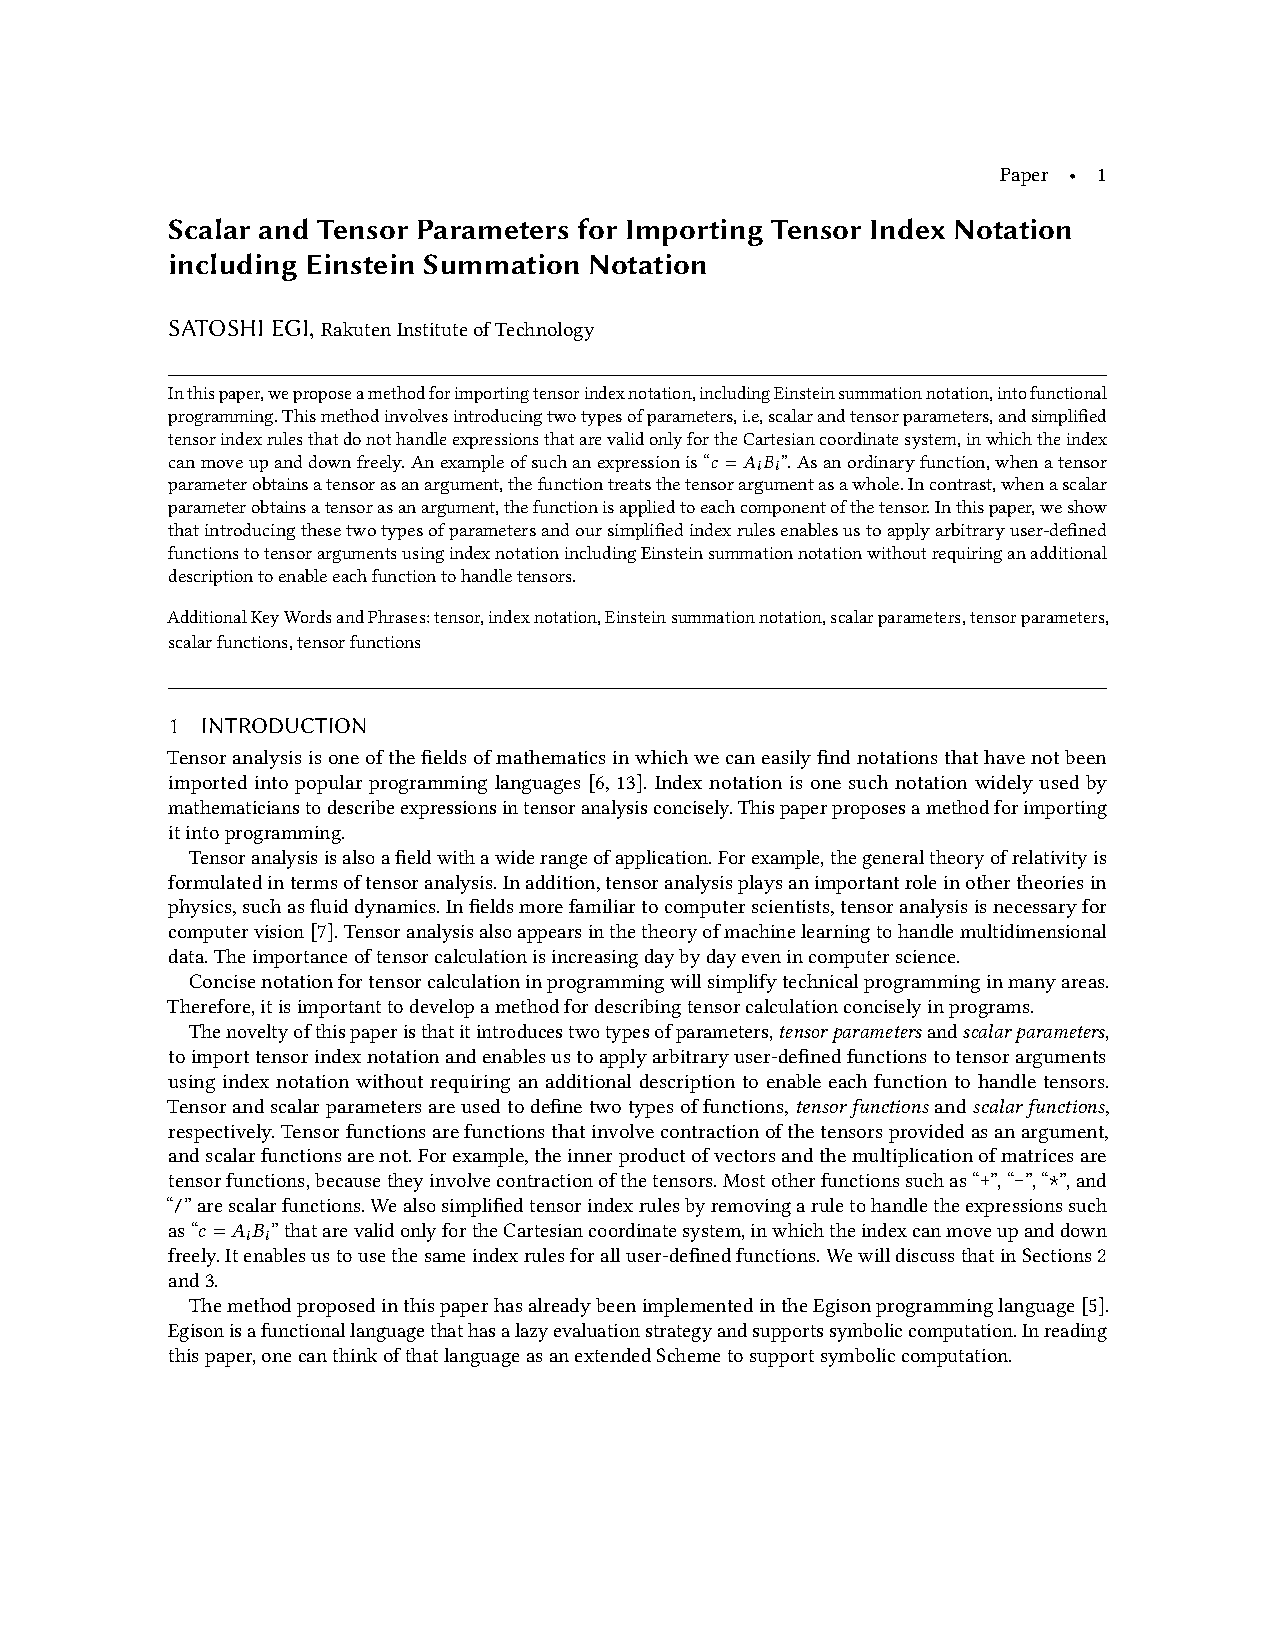
\includepdf[noautoscale,scale=1.07,pages=-,pagecommand={\thispagestyle{fancy}},addtotoc={1,chapter,1,{Paper: Scalar and Tensor Parameters for Importing Tensor Index Notation ...},egi}]{paper-egi}

\ \\
\pagebreak

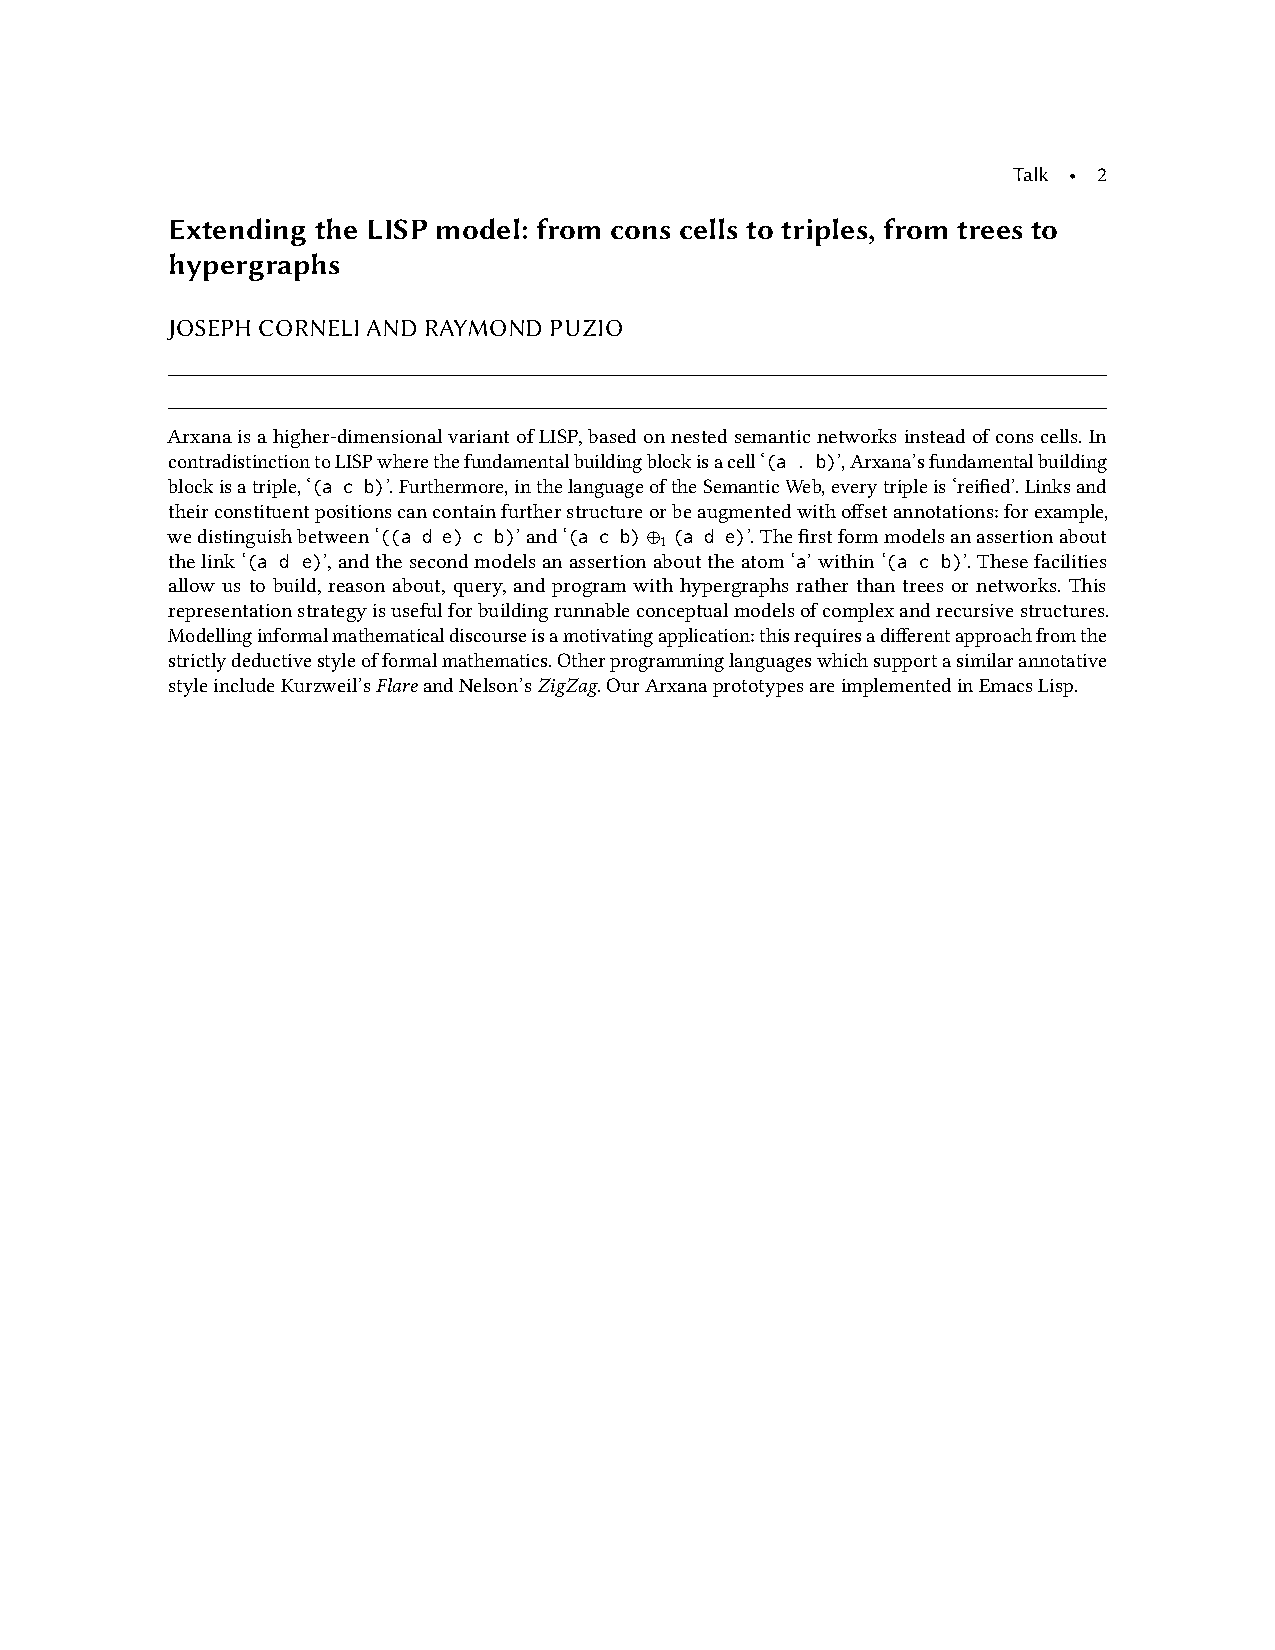
\includepdf[noautoscale,scale=1.07,pages=-,pagecommand={\thispagestyle{fancy}},addtotoc={1,chapter,2,{Talk:\ \ \ Extending the LISP model from cons cells to triples, from trees to hypergraphs},arxana}]{talk-arxana}

\ \\
\pagebreak

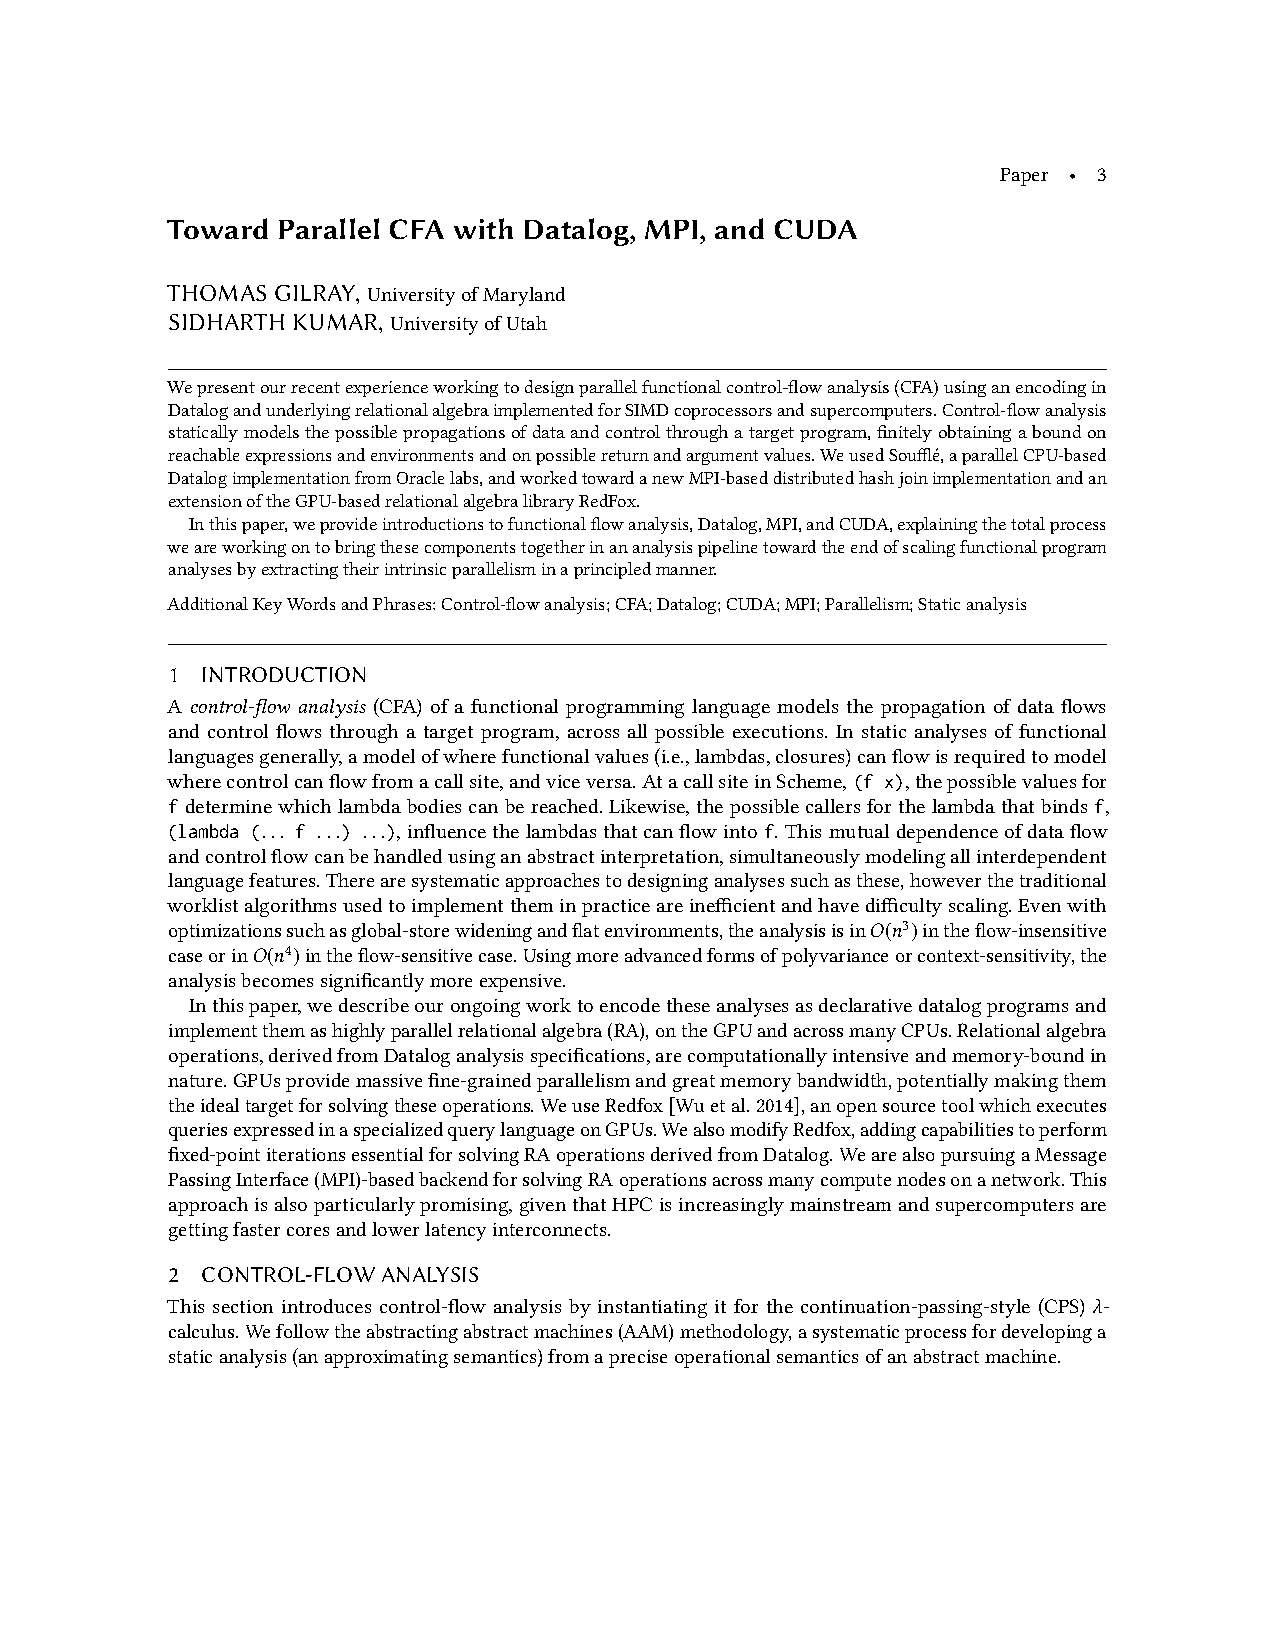
\includepdf[noautoscale,scale=1.07,pages=-,pagecommand={\thispagestyle{fancy}},addtotoc={1,chapter,3,{Paper: Toward Parallelizing Control-flow Analysis with Datalog},gilray}]{paper-gilray}

\ \\
\pagebreak

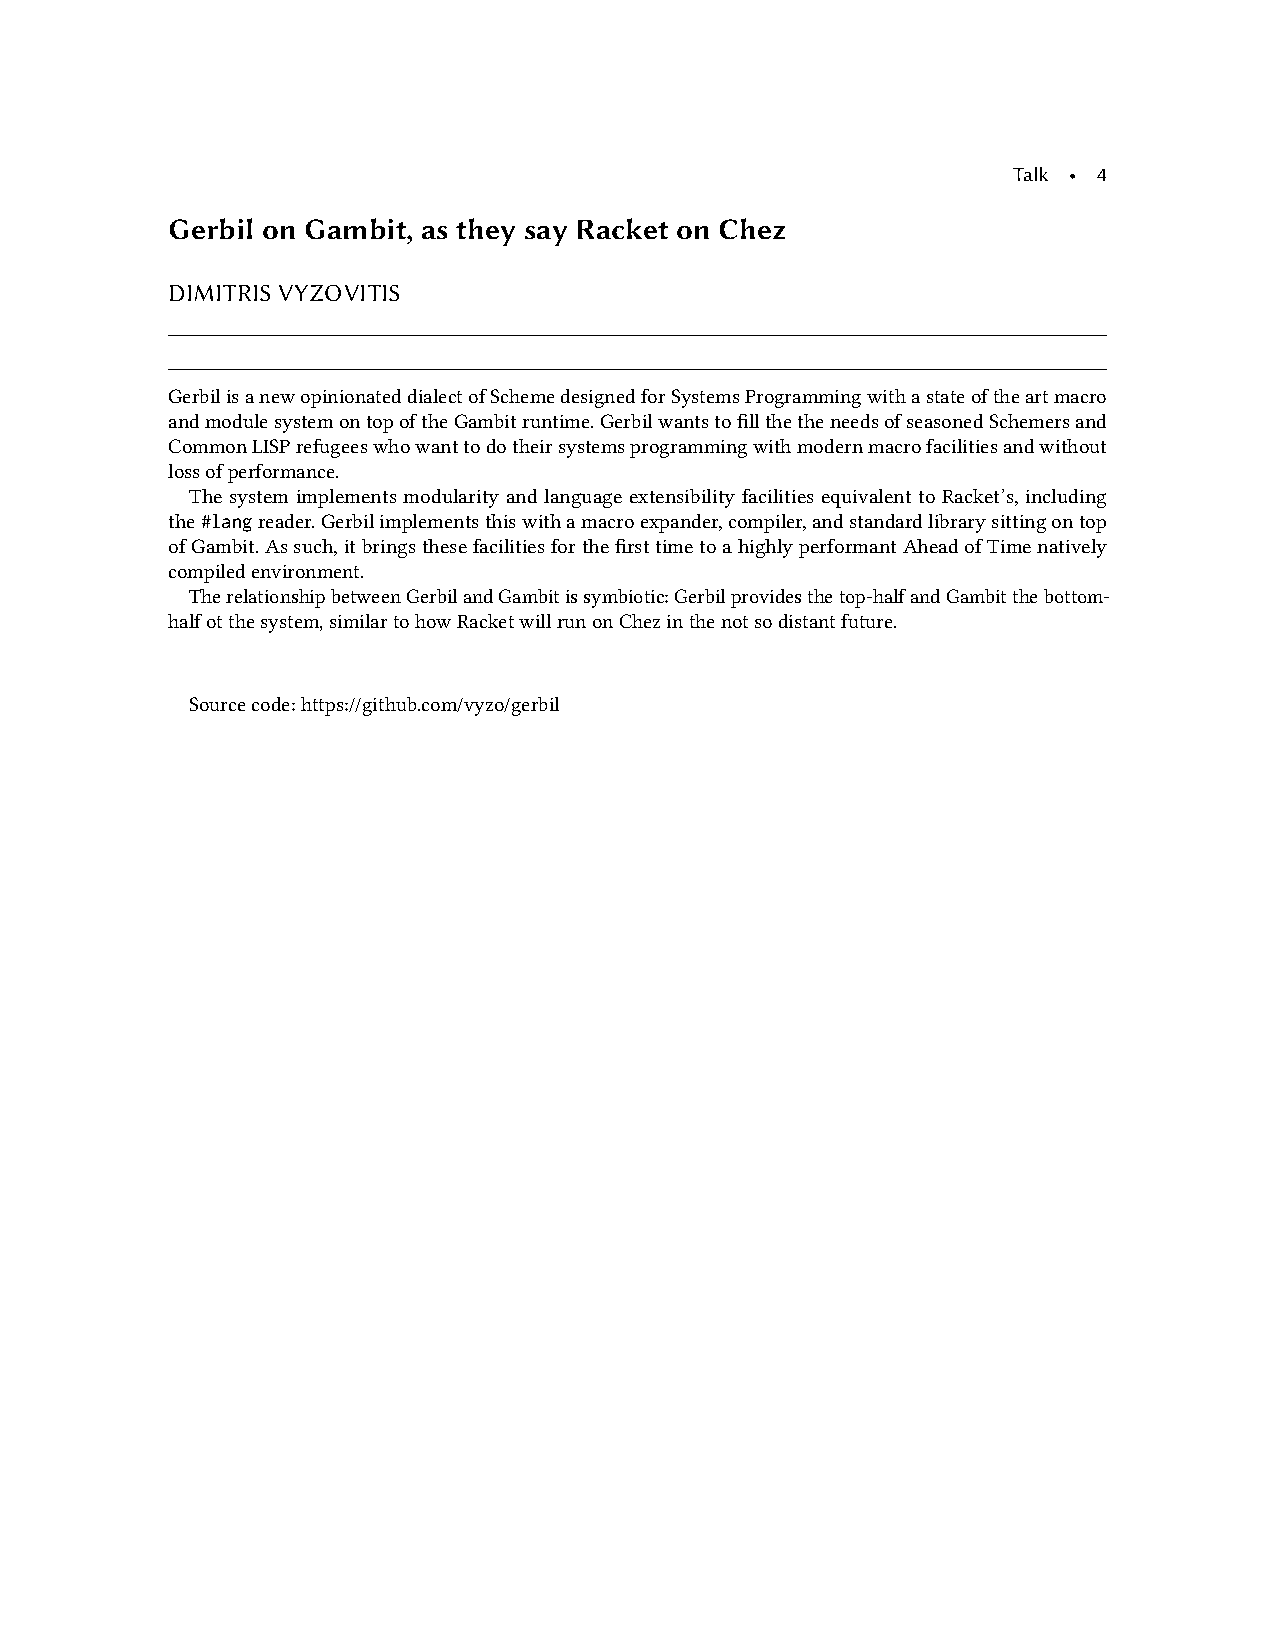
\includepdf[noautoscale,scale=1.07,pages=-,pagecommand={\thispagestyle{fancy}},addtotoc={1,chapter,4,{Talk:\ \ \ Gerbil on Gambit, as they say Racket on Chez},gerbil}]{talk-gerbil}

\ \\
\pagebreak

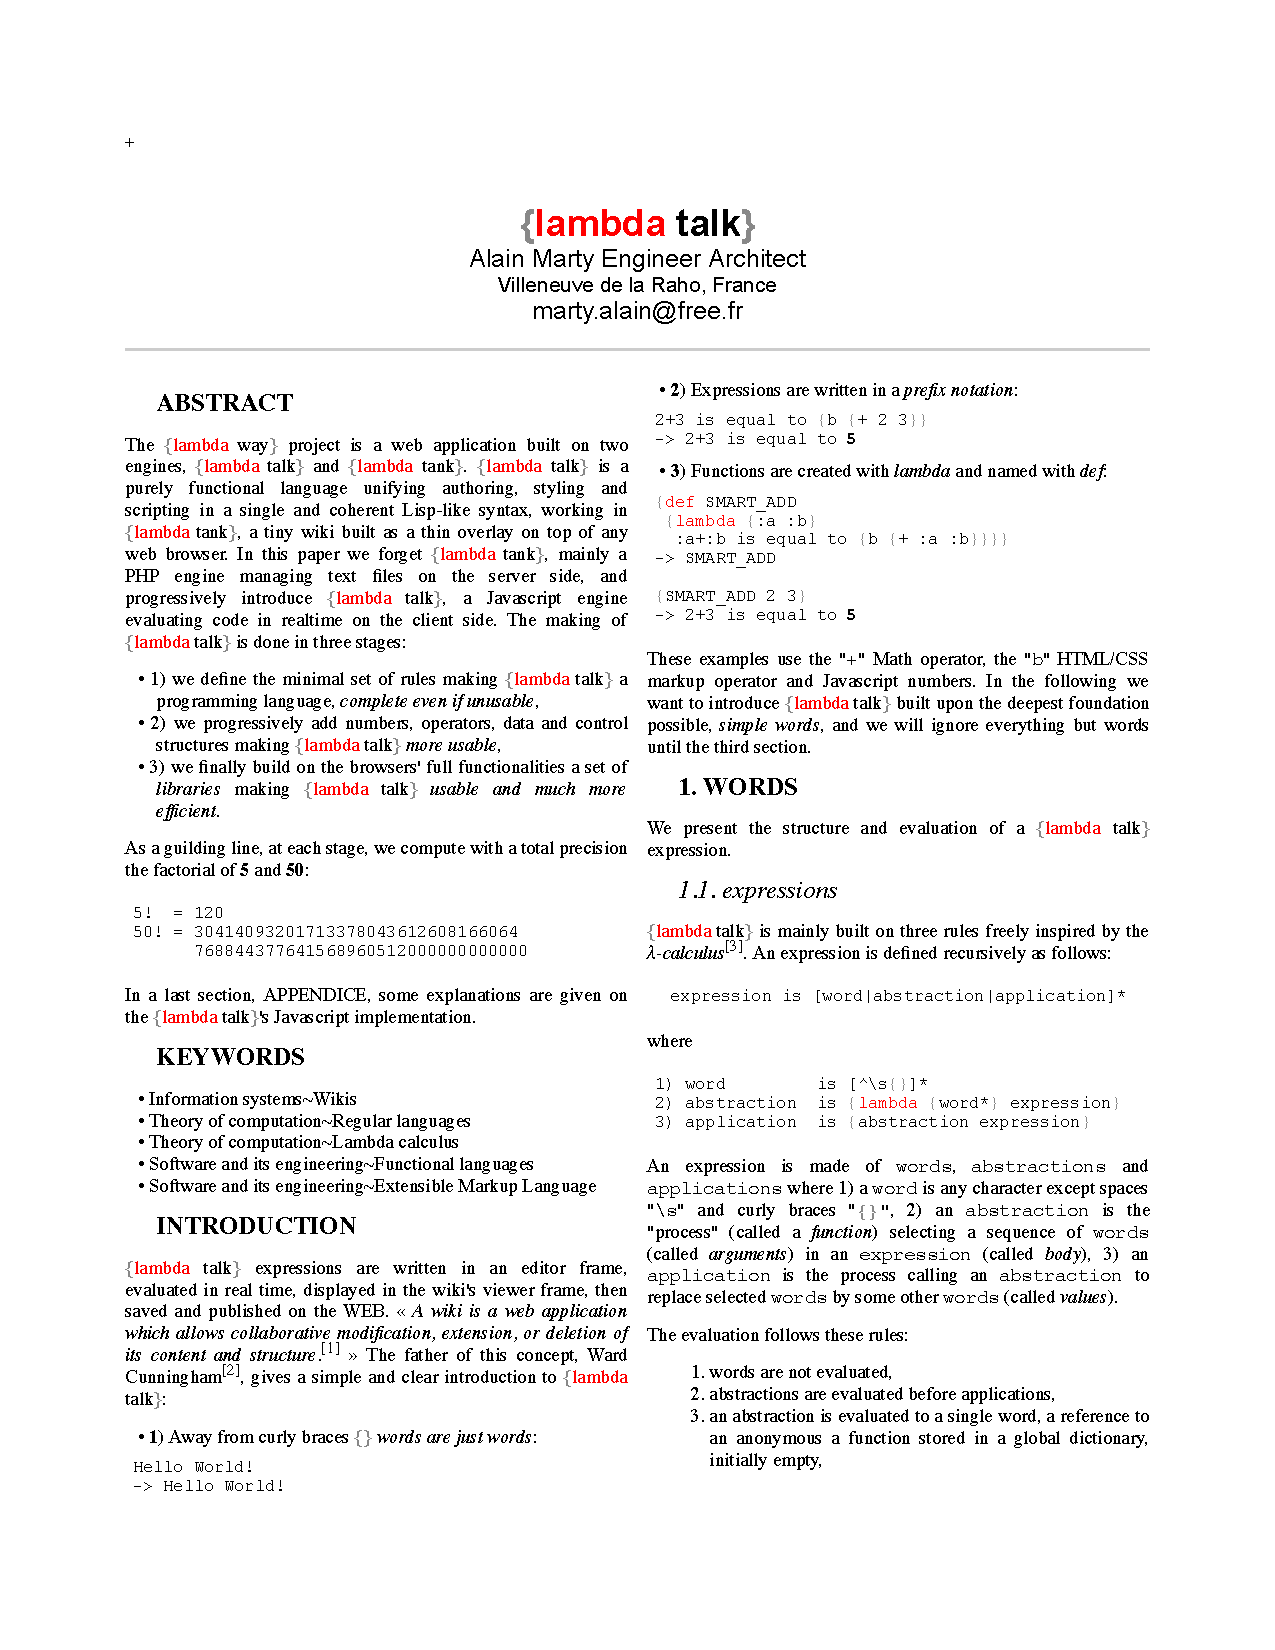
\includepdf[noautoscale,scale=0.98,pages=-,pagecommand={\thispagestyle{fancy}},addtotoc={1,chapter,5,{Talk:\ \ \ \{lambda talk\}},lambdatalk}]{talk-lambdatalk}
\end{document}
